%!TEX encoding = UTF-8 Unicode
%!TEX root = ../lect-w06.tex

%%%



\Subsection{Undantag}

\ifkompendium\else
\begin{SlideExtra}{Undantag kan orsaka krasch...}
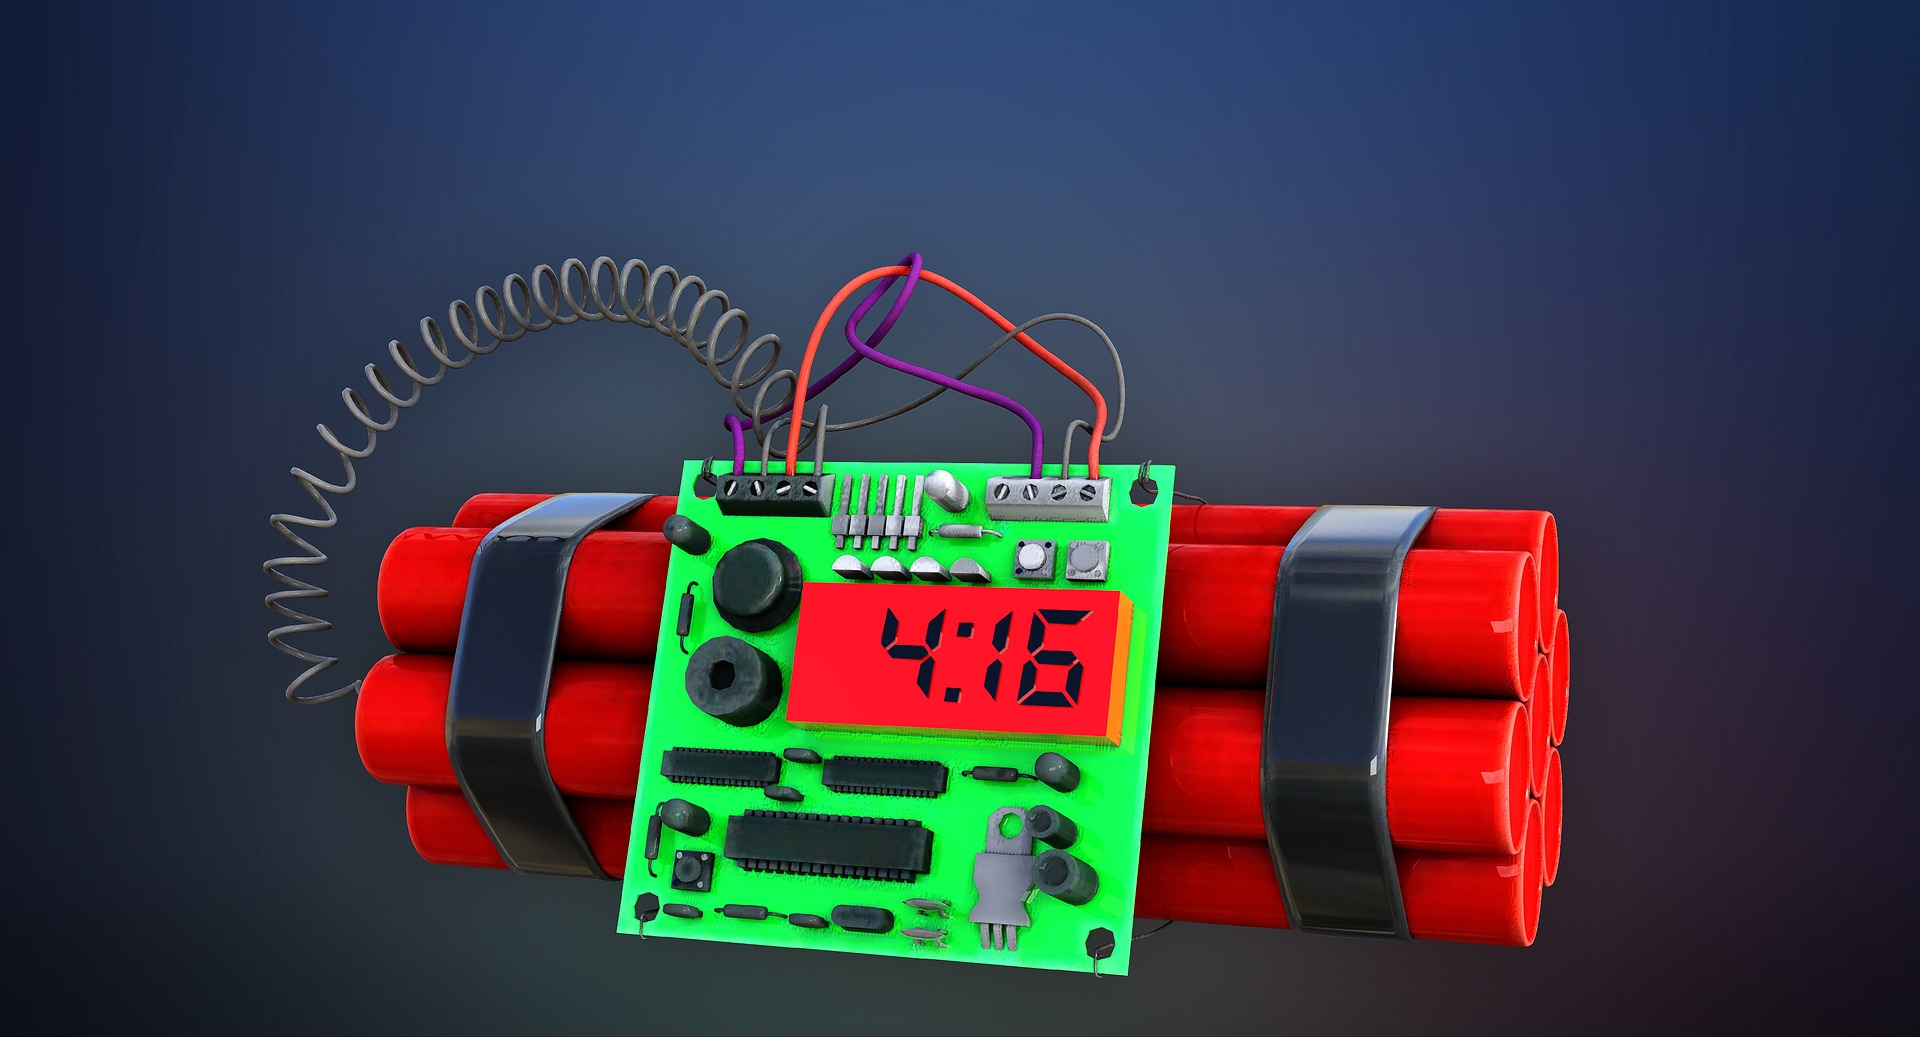
\includegraphics[width=1.0\textwidth]{../img/dynamite}  
\end{SlideExtra}

\begin{SlideExtra}{Undantag orsakar ingen krasch om inkapslad i en Try}
\hspace{0.3\textwidth}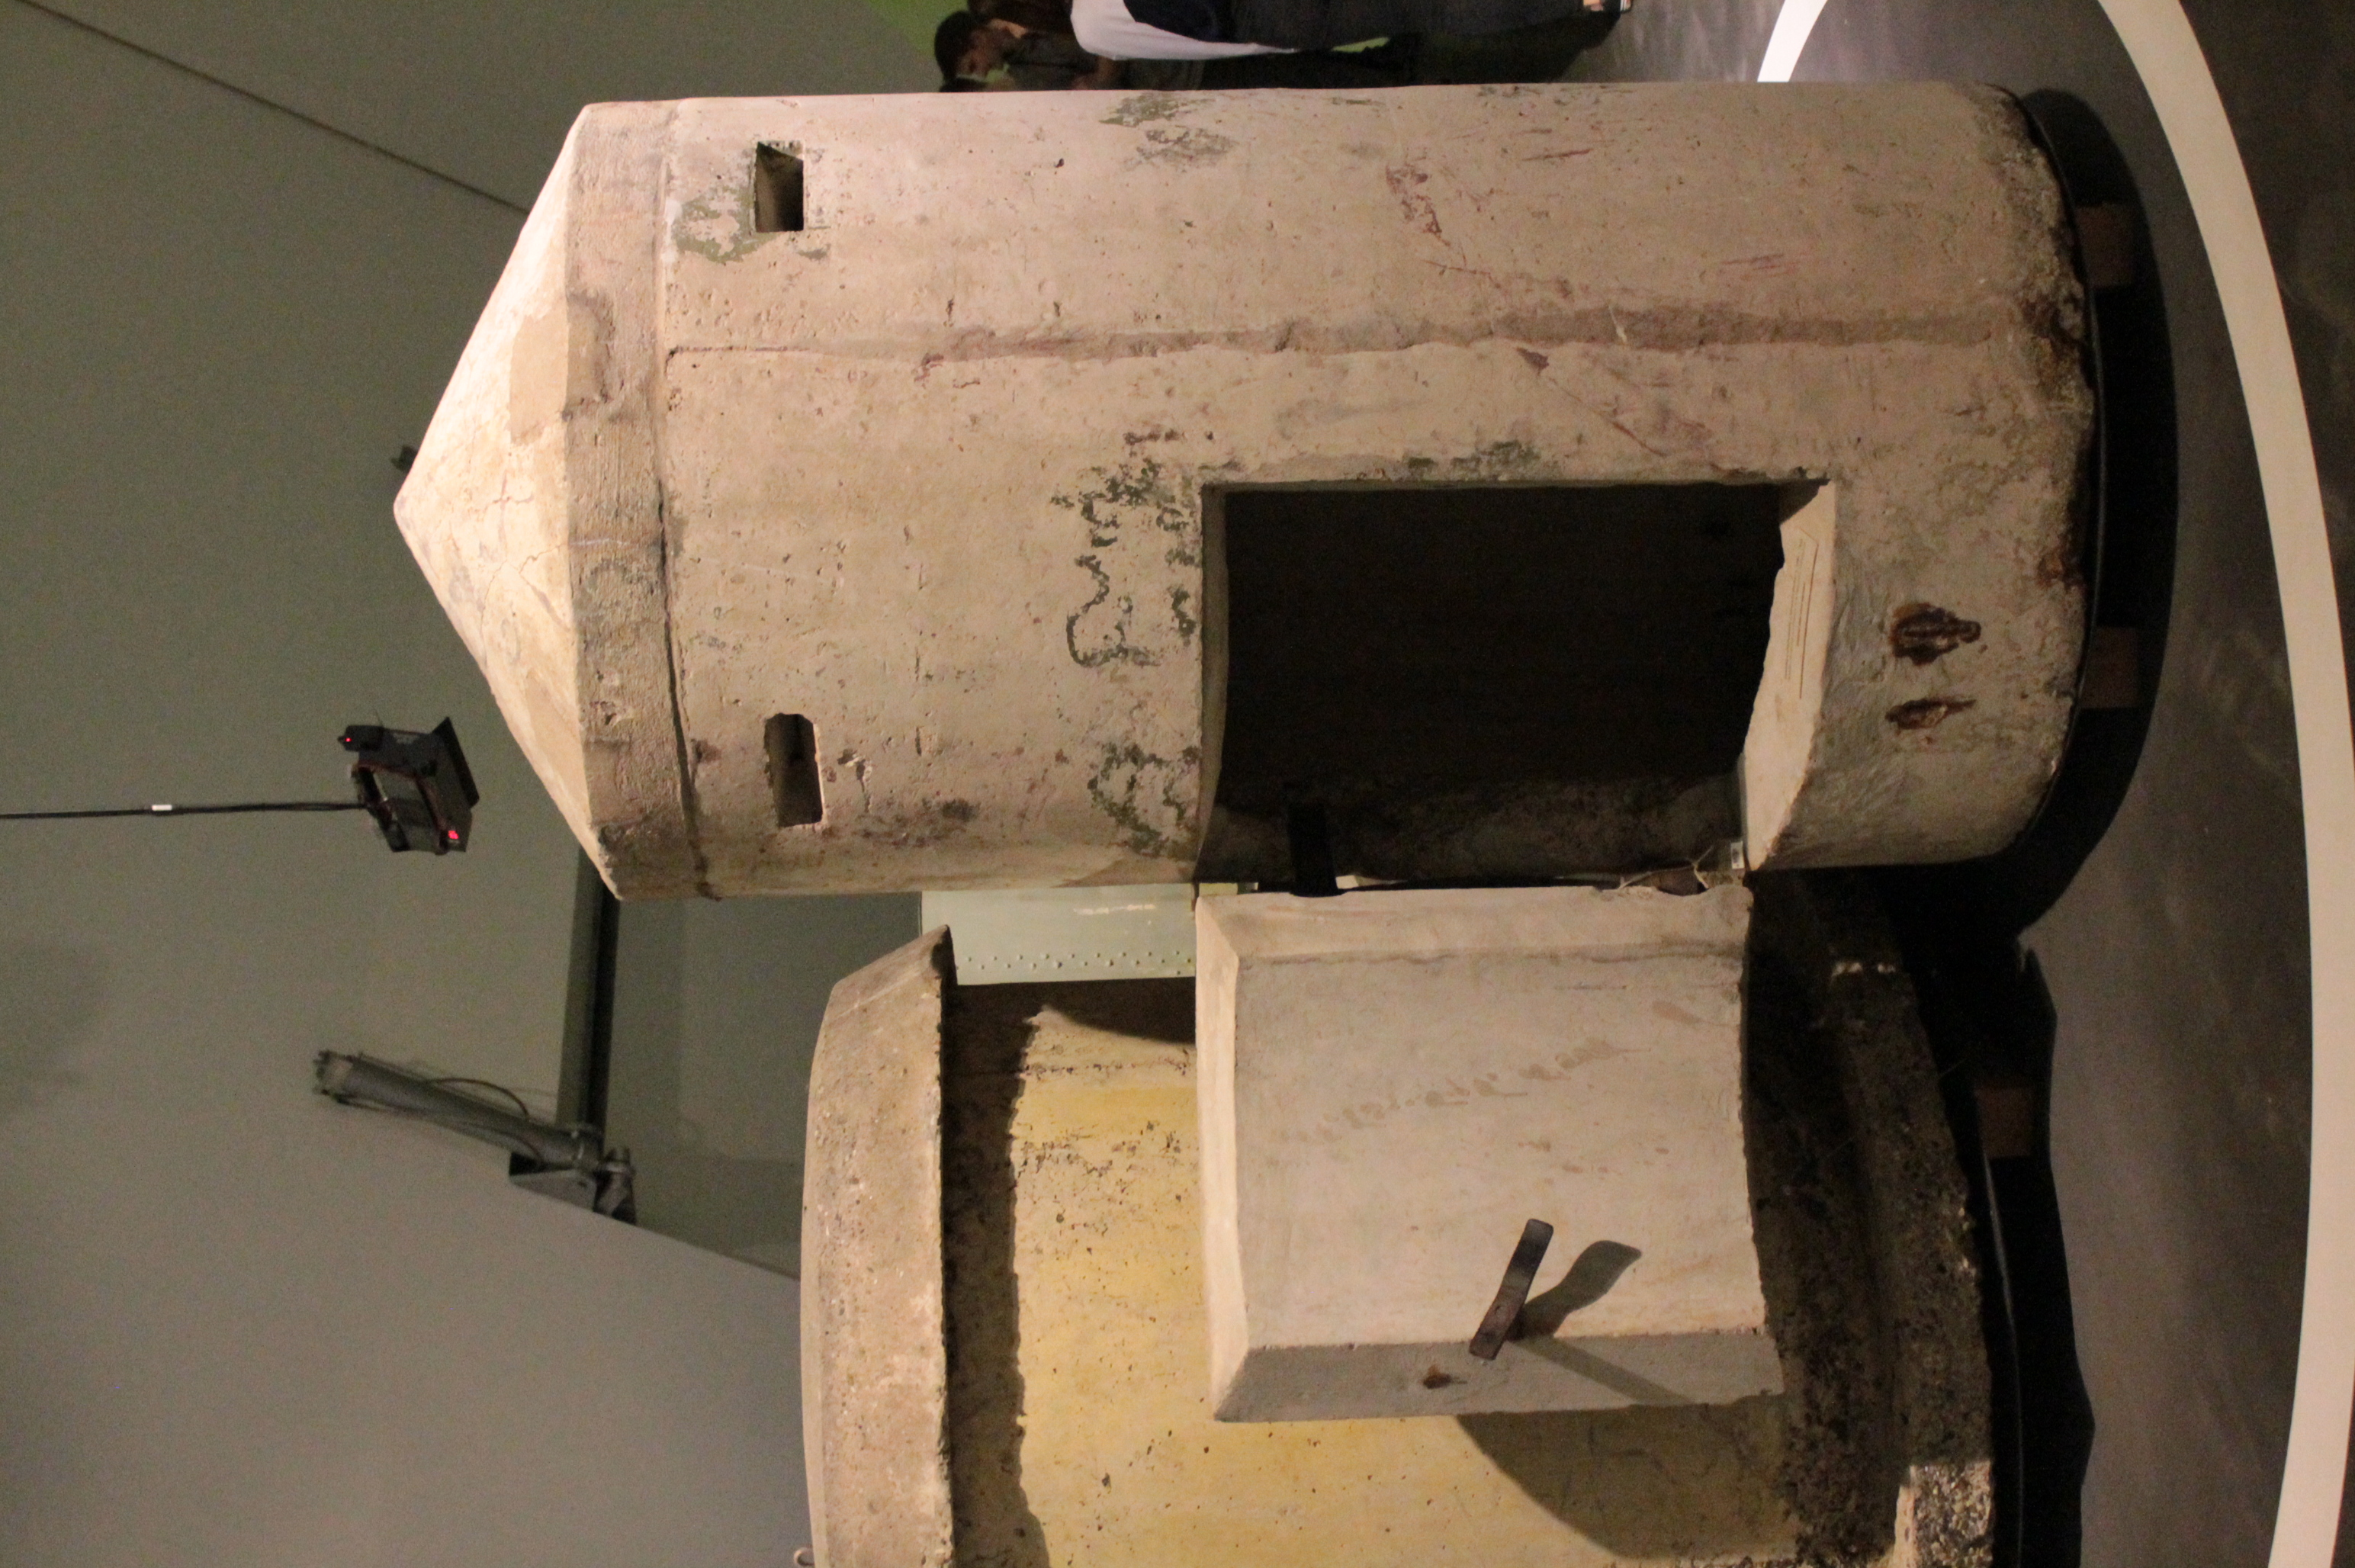
\includegraphics[width=0.6\textwidth,angle=-90,origin=c]{../img/bomb-shelter}  
\end{SlideExtra}
\fi

\begin{Slide}{Vad är ett undantag \Eng{exception}?}
Undantag representerar ett fel eller ett onormalt tillstånd som upptäcks under exekvering och som  behöver hanteras på särskilt sätt vid sidan av det normala exekveringsflödet.

\vspace{1em}\href{https://sv.wikipedia.org/wiki/Undantagshantering}{sv.wikipedia.org/wiki/Undantagshantering}


\vspace{1em} Exempel på undantag:

\pause

\begin{itemize} \SlideFontSmall
\item Indexering utanför vektorns indexgränser.

\item Läsning bortom filens slut.

\item Försök att öppna en fil som inte finns.

\item Minnet är slut.

\item Heltalsdivision med noll ger \code{java.lang.ArithmeticException}.

\item \code{"hej".toInt} ger \code{java.lang.NumberFormatException}

\end{itemize}

\end{Slide}


\begin{Slide}{Orsaka undantag indirekt med \texttt{require} och \texttt{assert}}

\begin{itemize}\SlideFontSmall
  \item Med funktionen \code{require(p)} skapas ett \code{IllegalArgumentException("requirement failed")} \\ om \code{p} är \code{false}
  \item \code{require} används om man vill begränsa vilka argument som är giltiga
  \item Med funktionen \code{assert(p)} skapas ett \code{AssertionError("assertion failed")} \\ om \code{p} är \code{false} 
  \item \code{assert} används om man vill förhindra ogiltiga tillstånd
\end{itemize}
{
  \ifkompendium\else
  \vfill\SlideFontTiny
  \fi
  Se implementationen av \code{require} här:\\
\url{https://github.com/scala/scala/blob/v2.13.6/src/library/scala/Predef.scala#L315}
}
\end{Slide}

\begin{Slide}{Kasta dina egna undantag med \texttt{throw}}\SlideFontSmall
Man kan själv generera ett undantag med \code{throw}, vilket kallas att \Emph{kasta} ett undantag som (om det inte \Emph{fångas}), gör att exekveringen \Alert{avbryts}.


\begin{REPL}
scala> def pang = throw Exception("PANG!")
pang: Nothing

scala> pang
java.lang.Exception: PANG!

\end{REPL}
\pause
Olika sätt att hantera undantag och förhindra att exekveringen avbryts:
\begin{itemize}
\item \code{try catch}-uttryck omvandlar undantag till ngt lämpligt värde.
%\item Java: Man kan använda en \code{try ... catch}-sats och \Alert{göra något} i händelse av undantag.

\item \texttt{scala.util.Try} \Emph{kapslar in} kod som kan ge undantag.  %(Finns ej i Java; att föredra i Scala.)
\end{itemize}
\end{Slide}


\Subsection{Hantera undantag med \texttt{Try}}

\begin{Slide}{En gemensam bastyp för något som kan misslyckas}\SlideFontSmall
\begin{Code}
import scala.util.{Try, Success, Failure}
\end{Code}
\ifkompendium\footnotesize\fi
\vspace{-0.5em}\begin{center}
\newcommand{\TextBox}[1]{\raisebox{0pt}[1em][0.5em]{#1}}
\tikzstyle{umlclass}=[rectangle, draw=black,  thick, anchor=north, text width=3.0cm, rectangle split, rectangle split parts = 3]
\begin{tikzpicture}[inner sep=0.5em]
\node [umlclass, rectangle split parts = 2, xshift=0cm, text width=3.8cm] (BaseType)  {
            \textit{\textbf{\centerline{\TextBox{\code{Try[T]}}}}}
            \nodepart[]{second}
            \TextBox{\code{def get: T}}\newline
            \TextBox{\code{def isFailure: Boolean}}\newline
            \TextBox{\code{def isSuccess: Boolean}}
        };

\node [umlclass, rectangle split parts = 2, text width=2.2cm]  at (-2.5cm,-3.7cm) (SubType1) {
            \textbf{\centerline{\TextBox{\code{Success[T]}}}}
            \nodepart[]{second} \TextBox{\code{val value: T}}
        };

\node [umlclass, rectangle split parts = 2, text width=4.2cm] at (2.5cm,-3.7cm) (SubType2)  {
            \textbf{\centerline{\TextBox{\code{Failure[T]}}}}
            \nodepart[]{second} \TextBox{\code{val exception: Throwable}}
        };
\draw[umlarrow] (SubType1.north) -- ++(0,0.5) -| (BaseType.south);
\draw[umlarrow] (SubType2.north) -- ++(0,0.5) -| (BaseType.south);
\end{tikzpicture}
\end{center}
\end{Slide}

\begin{Slide}{Hantera undantag med \texttt{Try}}
\vspace{-0.5em}\begin{REPLsmall}
scala> def pang = throw new Exception("PANG!")

scala> def kanskePang = if math.random() < 0.5 then 42 else pang

scala> import scala.util.{Try, Success, Failure}

scala> def försök = Try { kanskePang }

scala> val xs = Vector.fill(15){försök}

scala> val trettonde = xs(12) match
         case Success(value) => value
         case Failure(e) => println(e); -1

scala> (xs(12).isSuccess, xs(12).isFailure) 

scala> xs(12).getOrElse(0)

scala> xs(12).toOption

scala> försök.foreach(println)

scala> försök.map(_ + 1)

scala> for Success(x) <- xs yield x
\end{REPLsmall}
\end{Slide}

\Subsection{Hantera undantag med \texttt{try}-\texttt{catch}}


\begin{Slide}{\texttt{try}-\texttt{catch}-uttryck}\SlideFontSmall
Man kan fånga undantag med ett \code{try ... catch}-uttryck:
\begin{Code}
def carola = 
  try 
    if math.random() > 0.5 then throw Exception("stormvind")
    42
  catch 
    case e: Exception =>
      println("Fångad av en " + e.getMessage)
      -1

\end{Code}
\pause
\begin{REPL}
scala> Vector.fill(5)(carola)
Fångad av en stormvind
Fångad av en stormvind
Fångad av en stormvind
val res0: Vector[Int] = Vector(-1, 42, 42, -1, -1)
\end{REPL}
%Gör uppg. 9-11 i övn. \code{patterns} som visar hur man fångar undantag i Scala och Java. 
%Mer om undantag i fortsättningskursen.
\end{Slide}
